\documentclass[12pt,letterpaper]{article}
\usepackage[utf8]{inputenc}
\usepackage{graphicx} %Para importar gráficos
\usepackage[spanish, mexico]{babel} %Para que el contenido del documento esté en español de México
\usepackage[hidelinks]{hyperref} %Para el enlace al final del documento

\usepackage{pgfplots}

\author{Eduardo René Rodríguez Ávila}
\title{La integral (usando PGFPlots)}


\begin{document}
	
\maketitle

La integración es un concepto fundamental del cálculo y del análisis matemático. Básicamente, una integral es una generalización de la suma de infinitos sumandos, infinitamente pequeños.

\begin{figure}[h] 
	\centering
	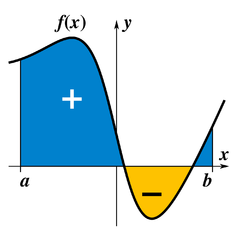
\includegraphics[width=0.4\textwidth]{img/integral_example.png}
	\caption{La integral definida de una función representa el área limitada por la gráfica de la función, en un sistema de coordenadas cartesianas con signo positivo cuando la función toma valores positivos y signo negativo cuando toma valores negativos.}
	\label{fig:uno}
\end{figure}

El cálculo integral, encuadrado en el cálculo infinitesimal, es una rama de las matemáticas en el proceso de integración o antiderivación, es muy común en la ingeniería y en la ciencia también; se utiliza principalmente para el cálculo de áreas y volúmenes de regiones y sólidos de revolución.

Fue usado por primera vez por científicos como Arquímedes, René Des\-car\-tes, Isaac Newton, Gottfried Leibniz e Isaac Barrow. Los trabajos de este último y los aportes de Newton generaron el teorema fundamental del cálculo integral, que propone que la derivación y la integración son procesos inversos.

\section{Teoría}

Dada una función $f(x)$ de una variable real x y un intervalo $[a,b]$ de la recta real, la integral

\begin{displaymath}
	\int_{a}^{b} f(x) \,\mathrm{d}x
\end{displaymath}



\noindent es igual al área de la región del plano $xy$ limitada entre la gráfica de $f$, el eje $x$, y las líneas verticales $x =a$ y $x =b$, donde son negativas las áreas por debajo del eje $x$.

\begin{figure}[h] 
	\centering
	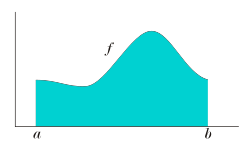
\includegraphics[width=0.7\textwidth]{img/area-under-curve.png}
	\caption{$\int_{a}^{b} f(x) \,\mathrm{d}x$ se interpreta como el área bajo la curva de $f$, entre $a$ y $b$.}
	\label{fig:dos}
\end{figure}



\section{Conceptos y aplicaciones}

Las integrales aparecen en muchas situaciones prácticas. Considérese una piscina. Si es rectangular y de profundidad uniforme, entonces, a partir de su longitud, anchura y profundidad, se puede determinar fácilmente el volumen de agua que puede contener (para llenarla), el área de la superficie (para cubrirla), y la longitud de su borde (si se requiere saber su medida). Pero si es ovalada con un fondo redondeado, las cantidades anteriores no son sencillas de calcular. Una posibilidad es calcularlas mediante integrales. 

Para el cálculo integral de áreas se sigue el siguiente razonamiento: 

\begin{enumerate}
	\item  Por ejemplo, consideremos la curva mostrada en la figura \ref{fig:tres}, gráfica de la función $y = f ( x ) = x^2$, acotada entre $x = 1$ y $x = 3$.
   \item  La respuesta a la pregunta ¿Cuál es el área bajo la curva de función $f$, en el intervalo desde 1  hasta 3? es: que el área coincidirá con la \textbf{integral} de  $f$. La notación para esta integral será $\int_{1}^{3} x^2 \,\mathrm{d}x$.
\end{enumerate}


\begin{figure}[h] 
	\centering

	\begin{tikzpicture}
	\begin{axis}[xmin=0, xmax=4, ymin=0, ymax=10, axis lines=middle, xlabel=$x$, ylabel=$y$]
		\addplot[domain=0:4]{x^2};
		\addplot[domain=1:3,fill=green!20!yellow]{x^2}\closedcycle;
		\node at (axis cs:3.6,4.2){Área};
		\draw[<-](axis cs:3,4)--(axis cs:3.4,4);
	\end{axis}
\end{tikzpicture}

	\caption{Cálculo del área bajo la curva (gráfico usando PGFPlots)}
	\label{fig:tres}
\end{figure}

Una primera aproximación, aunque no muy precisa, para obtener esta área, consiste en determinar el área del cuadrado unidad cuyo lado lo da la distancia desde $x=1$ hasta $x=3$ o también la longitud entre $y=f(1)=1$ y $y=f(3)=0$. Su área es exactamente $2 \times 9 = 18$. Tal como se puede inferir, el verdadero valor de la integral tendrá que ser más pequeño. Particionando la superficie en estudio, con trazos verticales, de tal manera que vamos obteniendo pequeños rectángulos, y reduciendo cada vez más el ancho de los rectángulos empleados para hacer la aproximación, se obtendrá un mejor resultado. Por ejemplo, dividamos el intervalo en cinco partes, empleando los puntos 1, $\frac{3}{2}$, 2, $\frac{5}{2}$ y finalmente la abscisa 3. Se obtienen cinco rectángulos cuyas alturas se determinan aplicando la función con las abscisas anteriormente descritas (del lado derecho de cada pedazo de la curva), así $1^2$, $(\frac{3}{2})^2$, $2^2$... y así hasta $3^2$. Sumando las áreas de estos rectángulos, se obtiene una segunda aproximación de la integral que se está buscando,

\[
 1^2(1^2 - 0)+ \left(\frac{3}{2}\right)^2\,\left(\frac{3}{2}- 1\right)+ \dots + 3^2\left(3-\frac{5}{2}\right) \approx 11.75
\]

Nótese que se está sumando una cantidad finita de valores de la función $f$, multiplicados por la diferencia entre dos puntos de aproximación sucesivos. Se puede ver fácilmente que las continuas aproximaciones continúan dando un valor más grande que el de la integral. Empleando más pasos se obtiene una aproximación más ajustada, pero no será nunca exacta. La solución utilizando el cálculo real de integrales, sería por otro lado:

\begin{displaymath}
	A = \int_{1}^{3} x^2 \mathrm{d}x = \left.\frac{x^3}{3}\right |_1^3 = \frac{27}{3} - \frac{1}{3} \approx 9.66 u^2
\end{displaymath}



Más información en: \url{http://es.wikipedia.org/wiki/Integraci\%C3\%B3n}
\end{document}